\documentclass[11pt,letterpaper]{article}

\usepackage[latin1]{inputenc}

\usepackage{fullpage}
\usepackage{graphicx}
\usepackage{enumitem}
\usepackage{caption} 
\usepackage{hyperref} 
\usepackage{array}
\usepackage{amsmath}
\usepackage{amssymb}
\usepackage{booktabs}

\begin{document}


\title{Multimodal Agents for Autonomous Interaction with Graphical User Interfaces}

\author{%
Ruijie Chen, Haotian Hao, Yuhan Huang, Shufeng Yin, Tianyi Zhou\\
{\small\begin{minipage}{\linewidth}\begin{center}
\begin{tabular}{ccc}
    $\{$ruijiech, ikun, hyuhan, shufengy, zhtianyi$\}$@umich.edu
\end{tabular}
\end{center}\end{minipage}}\\
}

%

\date{February 2025}


\maketitle





\section{Problem Statement \& Significance}

% What is the problem that you are trying to solve? Why is the problem important and interesting? What are things that are held back because your problem has not been solved yet? What are great things that could happen if you solved your problem?

In this fully digitized era, where personal electronic devices have become an essential aspect of one's work and life , the ability to automate everyday mundane action would drastically improve work efficiency. For instance, agent that can open inbox and send emails, sent up meetings, and mark events on a calendar. However, it is challenging to incorporate such an agent into a complex digital environment to recognize different elements of the UI and deliver a complete thinking chain. In this project, we build a VLM(Vision Language Model) agent capable of identifying UI(User Interface) elements and performing multistep tasks by automated mouse and keyboard actions based on user text prompt, with reflective features that make the pipeline align with intuitive human thought process.


\section{Related Work}

Recent advancements in vision-language-action (VLA) models and agent frameworks have laid the groundwork for autonomous GUI interaction. This section situates our work within the context of five research directions, synthesizing foundational contributions and identifying critical gaps.

\subsection{Frameworks}
Prior frameworks face three key limitations: Platform dependency, exemplified by OS-Copilot's API-driven Windows control and NNetscape Navigator's DOM-based web automation, which fail on unseen interfaces; Fragmented task tracking, where hierarchical memory systems (Agent Workflow Memory) and state-aware planners (OSCAR) operate in isolation without shared context; Static reward mechanisms, as seen in Cradle's fixed reward templates, which cannot adapt to GUI state complexity. Recent efforts continual learning partially address memory fragmentation but rely on manual trajectory annotation. Our framework introduces a unified visual ontology that maps pixels to platform-agnostic interaction primitives (clicks, scrolls), coupled with a dynamic reward engine that auto-calibrates penalties for occlusion handling and multi-step dependencies.

\subsection{VLA models}
While Aguvis and SpiritSight achieve pixel-to-action mapping through vision transformers, they treat actions as isolated predictions (mean error: 42px) rather than temporally coherent sequences. Reinforcement learning methods such as guided VLM agents improve temporal consistency through process rewards, but suffer from sparse training signals ( 5\% reward coverage). Digi-Q's offline RL mitigates this with value-based action pruning, yet struggles with novel UI layouts (success rate drop: 37\% on macOS to Linux transfer). We will utilize different large language modelas backbone to extract spatial-semantic features.

\subsection{GUI grounding}
Early graphical user interface (GUI) analysis primarily relied on Document Object Model (DOM) parsing to extract UI elements from websites. \cite{shi2017world}. 
However, this approach is limited as DOM data is often unavailable in many environments, such as mobile applications and desktop software. To address this problem, researchers turned to computer vision techniques to interpret the UI screenshots directly. Screen2Words used deep learning to extract semantic descriptions from UI screenshots. \cite{wang2021screen2words}
Recent research leverages multimodal large language models (MLLMs) that integrate vision and language to enhance the localization and interaction of UI elements. These methods, e.g. SeeClick, UGround, operate solely on screenshots, eliminating the dependency on DOM. \cite{cheng2024seeclick}\cite{gou2024navigating}.
Our method introduces a novel UI state-aware grounding mechanism, leveraging real-time visual feedback from hover-induced UI changes to enhance recognition accuracy. Unlike prior approaches that rely solely on static UI appearance, our model dynamically detects hover-based UI state transitions, such as color inversion, background shifts, or highlight effects, which frequently occur when elements are interactively engaged. 

\section{Proposed Method}
%
\begin{figure}
    \centering
    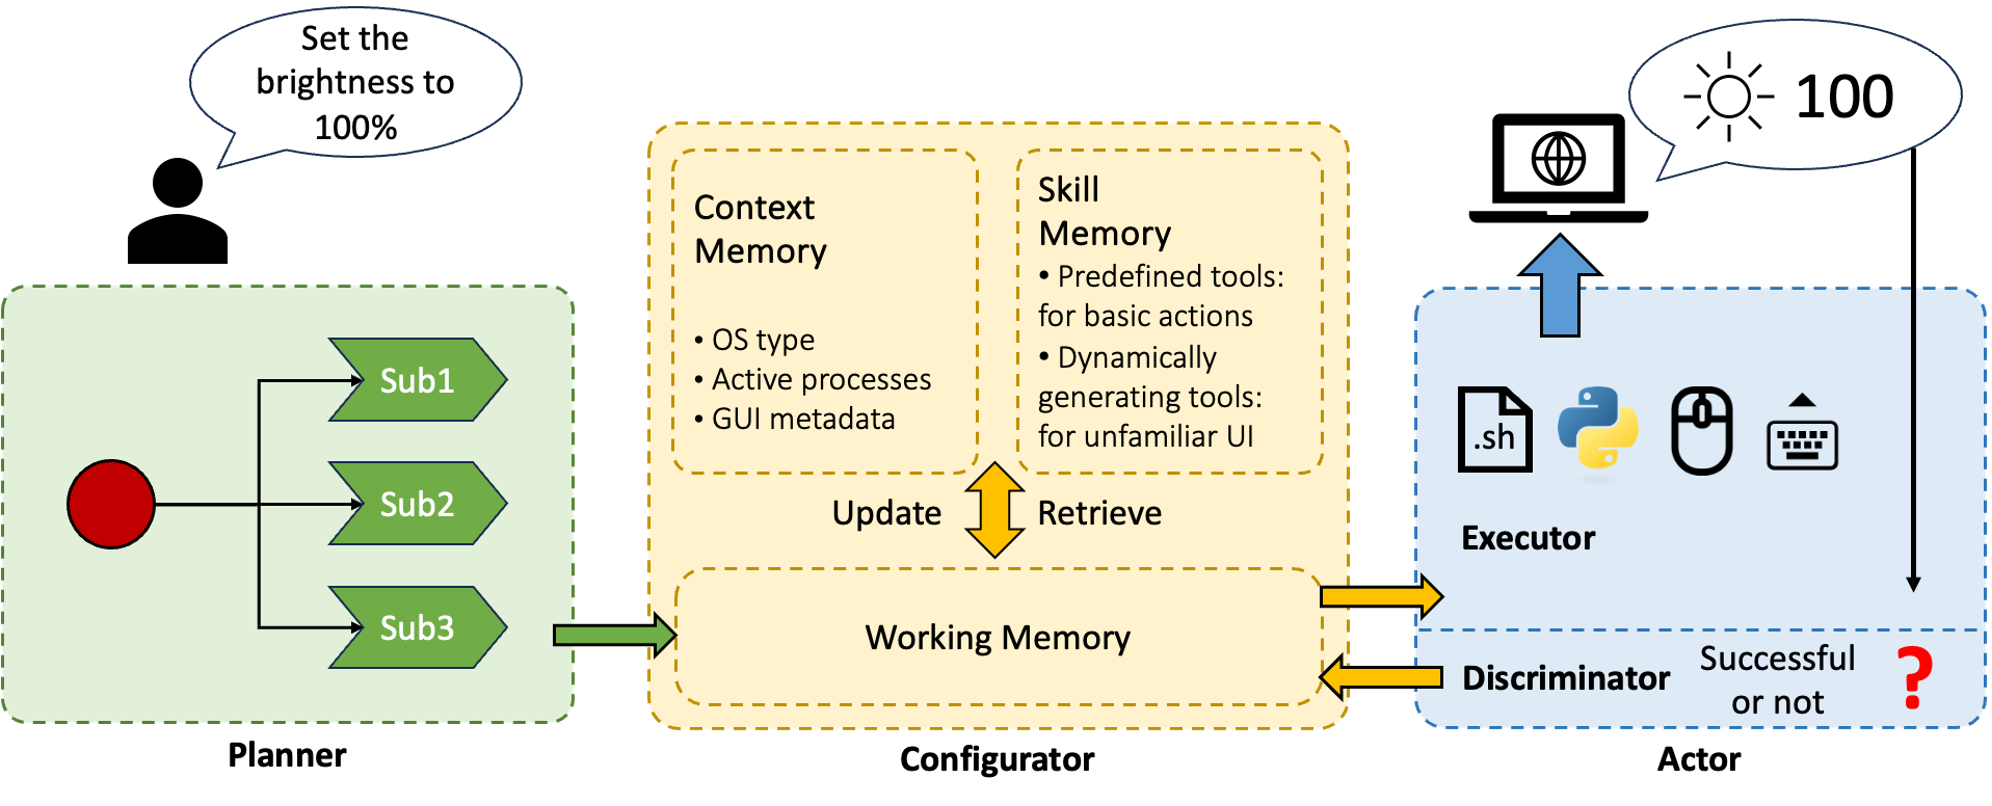
\includegraphics[width=0.8\linewidth]{framework.png}
    \vspace{-0.50cm}
    \caption{Overview of the proposed framework. }
    \vspace{-0.50cm}
    \label{fig:framework}
\end{figure}
%
As shown in Figure \ref{fig:framework}, the proposed framework consists three key components: 
%
a \textbf{planner} that decomposes the user request into subtasks; 
%
a \textbf{configuratior} that maintains a knowledge base for task completion; 
%
an \textbf{actor} that performs the operations to finish the tasks.
%

%
\subsection{Planner}
%
The planner decomposes complex user requests into simpler subtasks. 
%
It's critical for a planner to align the granularity of generated plan with the ability of the actor component.
%
To ensure its ability of reasoning and comprehending a wide range of user prompts, we plan to utlize LLM-based planner component. \cite{planandsolve}.
%
\subsection{Configurator}
%
The configurator serves as the adaptive core in the framework, dynamically bridging task decomposition in the planner and execution in the actor.
%
It is structured around three core memory systems: Context Memory, Skill Memory, and Working Memory.
%
\paragraph{Context Memory}
%
The context memory is a subcategory of long-term memory and stores static knowledge and real-time context.
%
It retains user preferences, such as preferred tools or frequently accessed applications. 
%
Additionally, it continuously updates real-time system states, including the operating system type, active processes, and GUI metadata.
%

\paragraph{Skill Memory}
%
The skill memory acts as a tool repository, including predefined tools for basic actions such as mouse interactions and text input and dynamically generating tools for unfamiliar applications.
%
When encountering an unlabeled UI element, the skill memory leverages LLMs to synthesize context-aware solutions, such as generating a keyboard shortcut sequence or writing a platform-specific script.
%
\paragraph{Working Memory}
%
The working memory handles real-time coordination between the planner and actor.
%
It retrieves relevant tools for subtasks and monitors execution feedback.
%
As the actor executes subtasks, the working memory monitors outcomes through real-time screenshots and system logs.
%
If the discriminator detects a Fail, the working memory initiates a reflection phase: a vision-language model (VLM) diagnoses issues and determines whether to retry with adjustments or request replanning.
%
\subsection{Actor}
% 
The actor consists of two stages: an executor that performs the subtask and a discriminator that judges the completion. 
%
\paragraph{Executor}
%
For a better cross-platform capability, we plan to design an encapsulated toolkit leveraging command-line scripts, Python program and input simulation. 
% 
Using the exceptional coding ability of state-of-the-art LLM models, the executor is able to flexibly choose and execute the optimal way of tackling the task.
%
\paragraph{Discriminator}
%
The discriminator judges whether the task has been completed successfully. 
%
Due to the lack of ground truth in this evaluation, we plan to gather the output of executor and the screenshot before and after the operation and utilize an LLM model to analyze the completion state.
%
\section{Experiment Results}
% How are you going to evaluate your method/approach? What is the evaluation metric or protocol? Which dataset or benchmark that you are going to use?

% We will use Visual Agent Bench \cite{Agentbench} to evaluate the performance of our model. The method consists of 8 different environment, in particular we will measure the agent performance in Operating System which is align with our expected task solving ability out of the model. This benchmark environment will generate human questions with deterministic answer in a interactive bash environment. The overall scores then are compared to existing models such as gpt-4, Claude etc. We will also create customized tests as a more fundamental metric report to measure the task completion rate, action efficiency(execution time taken, number of steps generated) . The other Evaluation method would be perceptual realism, we will create survey for user to report the correctness and response-ness of the model, how intuitive the agent performs under natural language interaction, how much work is delegated by using agent.
%
We choose ScreenAgent\cite{screenagent} and OS-Copilot\cite{wu2024copilot} as our baselines and conducted experiments on them. Here we report our preliminary experiments result and analysis on failure cases.
%
\subsection{Results on ScreenAgent}
%
We conducted experiments to replicate the results of ScreenAgent. 
%
We established a controlled desktop operating system environment in Docker container; configured and deploying the controller code execution environment; leveraged GPT-4o as LLM backend.
%
% The controller will collect the current screen image, fill in the prompt word template, send the image and complete prompt words to the large model inferencer, parse the reply from the large model inferencer, send mouse and keyboard control commands to the VNC Server, and complete tasks directly on the desktop.

% \vspace{10pt}

\noindent We conducted comprehensive testing across a dataset including 13 predefined tasks. 
%
We categorized the tasks in 3 levels of complexity by the number of operational steps required. 
%
The detailed outcomes of the tasks are summarized in Table \ref{tab:task_results}

\begin{table}[htbp]
\centering
\begin{tabular}{|p{6cm}|c|p{6cm}|}
\hline
\textbf{Task} & \textbf{Level} & \textbf{Result (Reason if failed)} \\
\hline
Open Firefox browser & 1 & \textbf{SUCCESS} \\
\hline
Open MousePad & 1 & \textbf{SUCCESS} \\
\hline
Open URL: https://Amazon.com & 2 & \textbf{SUCCESS} \\
\hline
Search product: ``MacBook Air with M4 chip" & 2 & \textbf{SUCCESS} \\
\hline
Open Google Chrome & 3 & \textbf{FAIL} (Fails to control Start Menu) \\
\hline
Open terminal and run command \texttt{source ./bashrc} & 3 & \textbf{FAIL} (Fails to control Start Menu) \\
\hline
Use MousePad to write paragraph & 3 & \textbf{SUCCESS}\\
\hline
Write Fourier Transform in MousePad and save file & 3 & \textbf{FAIL} (Fails to click save button) \\
\hline
Install Python3.10 & 3 & \textbf{SUCCESS} \\
\hline
Determine this machine's Ubuntu version and record in MousePad & 3 & \textbf{FAIL} (Fails to close window, desktop messed up) \\
\hline
Calculate 7*9 using web calculator & 3 & \textbf{FAIL} (Incorrect clicks on digits) \\
\hline
Search YouTube for Cooking Tutorials, play top video & 3 & \textbf{FAIL} (Fails to click filter button) \\
\hline
\end{tabular}
\caption{Testing result and reasons of failure cases of ScreenAgent.}
\label{tab:task_results}
\end{table}

\vspace{10pt}

\noindent Our experimental results show that ScreenAgent, integrated with GPT-4o, is capable of executing desktop automation tasks. The successful replication of ScreenAgent functionality demonstrates the viability of an automated approach in controlled desktop environments for simple tasks (Levels 1 and 2). However, challenges in accurately interacting with specific GUI elements (level 3 tasks) indicate areas needing improvement, particularly in the precision of GUI element interaction.

\subsection{Results on OS-Copilot(FRIDAY)}
OS-Copilot is a framework for building AI agents that can carry out a broad range of computer-based tasks, such as browsing the web, using code terminals, manipulating files, working with multimedia, and operating third-party apps. 

\vspace{10pt}

\noindent FRIDAY is a specific agent, designed on top of OS-Copilot, which can learn new skills through self-directed exploration and refine its own tools and strategies based on feedback. 

\vspace{10pt}

\noindent We assigned different task on the locally deployed Friday using gpt-3.5-turbo-0125 as the backend LLM model and obtained some preliminary result \ref{table:excel_tasks}. Overall, the agent is able to perform common file handling and basic excel manipulation pretty well, but we have not been able to explore the self-learning functionality of the model, which should exhibit when the model is assigned with task that is beyond its capability.

\vspace{10pt}

% \begin{minipage}{\textwidth} % This ensures it behaves like a floating object
%     \label{list:excel_tasks}  % Label to reference later
%     \begin{enumerate}[leftmargin=*]

%         \item \textbf{Query:} Copy any text file located in the working\_dir/document directory (by findstr command, not grep) that contains the word 'agent' to a new folder named 'agents'.  
%         \textbf{Nature of task:} Basic  
%         \textbf{Method:} Script-based  
%         \textbf{Result:} \textbf{SUCCESS}  

%         \item \textbf{Query:} You need to sort the data in Sheet1 of the Excel file based on the values in column C in ascending order. Ensure that the entire row is sorted accordingly. Save the sorted data back into the same file.  
%         \textbf{Nature of task:} Excel  
%         \textbf{Method:} Script-based  
%         \textbf{Result:} \textbf{SUCCESS}  

%         \item \textbf{Query:} Create a pivot table in Sheet2 using the data from Sheet1. Use 'Category' as the row field and 'Sales' as the values field with the sum function. Save the updated file.  
%         \textbf{Nature of task:} Excel  
%         \textbf{Method:} Script-based  
%         \textbf{Result:} \textbf{SUCCESS}  

%         \item \textbf{Query:} You need to do some tasks related to Excel manipulation. My sheet records data from an experiment where one hanging block (m2) drags a block (m1=0.75 kg) on a frictionless table via a rope around a frictionless and massless pulley. It has a sheet called Sheet1. Your task is: Fill out the rest of the rows in column B using the formula in B2. Create a scatter chart in Sheet1 with acceleration on the y-axis and the hanging mass on the x-axis. Add the corresponding column headers as the axis labels. You should complete the task and save the result directly in this Excel file.  
%         \textbf{Nature of task:} Excel  
%         \textbf{Method:} Script-based  
%         \textbf{Result:} \textbf{FAIL:} Cannot create bar chart  

%         \item \textbf{Query:} My workbook records many invoices made on different dates. Copy the 'Sheet1' Product column to a new sheet 'Sheet2' and sort 'Sheet2''s Product column in ascending order.
%         \textbf{Nature of task:} Excel  
%         \textbf{Method:} Self-learning  
%         \textbf{Result:} \textbf{FAIL:} Self learning process ended up in an infinite loop or incorrect tool function generated.
%         % \captionsetup{type=table}  % Treat the list like a table for referencing
%         % \caption{Summary of Excel Task Execution}
%     \end{enumerate}
% \end{minipage}

\begin{table}[ht]
    \centering
    \renewcommand{\arraystretch}{1.3}
    \begin{tabular}{|p{6cm}|p{2cm}|c|p{5cm}|}
        \hline
        \textbf{Query} & \textbf{Nature of Task} & \textbf{Method} & \textbf{Result(Reason if failed)} \\ 
        \hline
        Copy text files using \texttt{findstr} containing 'agent' to a new folder & Basic & Script-based & \textbf{SUCCESS} \\ 
        \hline
        Sort data in Sheet1 by Column C in ascending order & Excel & Script-based & \textbf{SUCCESS} \\ 
        \hline
        Create a Pivot Table in Sheet2 using 'Category' as rows and 'Sales' as values (Sum) & Excel & Script-based & \textbf{SUCCESS} \\ 
        \hline
        Fill out Column B using B2's formula and create a scatter chart with acceleration (y-axis) and hanging mass (x-axis) & Excel & Script-based & \textbf{FAIL}\ (Cannot create bar chart) \\ 
        \hline
        Copy 'Product' column from Sheet1 to Sheet2 and sort it in ascending order & Excel & Self-learning & \textbf{FAIL}\ (Infinite loop or incorrect tool function) \\ 
        \hline
    \end{tabular}
    \caption{Testing result and reasons of failure cases of OS-Copilot.}
    \label{table:excel_tasks}
\end{table}

\subsection{Analysis on Failure Cases}
In addition to the results above, we analyze the potential reason for further improvements.
%

%
ScreenAgent uses simulated input as the major agent to control the operating system. 
%
However, it suffers from inaccurate coordinates generated by LLM backend and fails to control small UI elements (e.g. save button in a notepad). 
%
Furthermore, such drawback also limits its overall efficiency since it takes several loops to find the correct clicking coordinates, even in a simplest task like opening the browser.
%

%
OS-Copilot majorly uses shell commands to control the operating system. 
%
However, unless specified in prompt, it generates shell commands, which is incompatible with Windows. 
%

%
Furthermore, both baselines stuck in infinite loop if some of the steps in a task fails. 
%
Situations is even worse in ScreenAgent since the indefinitely repeated operations will mess up the user interface. 
%

\section{Future Milestone}
Based on preliminary experiments on baselines, we plan to construct a more reliable multi-modal agent for autonomous interactions on various operating systems. Our work will mainly based on OS-Copilot and make modifications in reference to ScreenAgent and other related works. Specifically, our milestone can be list as follow, each milestone lasts for two weeks.

% \subsection{OS-Copilot(FRIDAY)}

\subsubsection*{Milestone 1: Prompt Engineering \& Benchmark Alignment}
The main goal is to improve OS-Copilot's understanding and utilization of the operating system environment and standardize evaluation of OS-Copilot's performance and versatility.
%
One week will be dedicated to reviewing related works of benchmarks for autonomous agents, establishing a unified benchmark for evaluation and design our final plan for experiments.
%
Another week will be dedicated to developing a module that automatically collects OS-specific information to optimize tool selection and integrating advanced prompt engineering techniques into the OS-Copilot framework and validating cross-platform consistency.

\subsubsection*{Milestone 2: Fine-Tuning Self-Learning Module}
The main goal is to prevent Self Learning module from falling into infinite loop and improve system stability and responsiveness. 
%
One week will be dedicated to implementing a timeout mechanism, where tasks will have predefined execution time and retry limits. 
%
Tasks exceeding these constraints will be immediately terminated, accompanied by warnings and corresponding log records. 
%
Additionally, a penalty mechanism to reduce the retry priority or extend the retry intervals for repeatedly failing tasks, thus preventing frequent recurrence of problematic tasks.

\section{Conclusion}
ScreenAgent is capable of executing simple desktop automation tasks, and it needs improvement to complete complex tasks, particularly in the precision of GUI element interaction.
%
FRIDAY's can handle files and manipulate Excel effectively but its self-learning functionality has yet to be tuned/explored.

\vspace{10pt}

\noindent In the future work, we plan to construct a more reliable autonomous agent mainly based on OS-Copilot and introduce automatic OS-based tool selection to improve it's cross-platform compatibility and eliminate the effects of infinite loops on failed tasks to enhance overall system stability
%
Furthermore, we will re-design the evaluation benchmark and present more comprehensive experiment results.
%
% \vspace{10pt}
% \noindent In future work, we will introduce automatic OS-based tool selection and standardized benchmarks to optimize OS-Copilot's performance evaluation. 
%
% Additionally, timeout and penalty mechanisms will be implemented in the Self-Learning module to prevent infinite loops and enhance overall system stability.

\bibliographystyle{IEEEtran}
\bibliography{refs}

\section*{\LARGE Appendix}
\section*{Contributions}

Ruijie Chen conceived the experiment for ScreenAgent and carried it out with Shufeng Yin. Haotian Hao carried out Haotian Hao and Yuhan Huang carried out experiments for OS-Copilot. Yuhan Huang further investigated Self-Learning Module of OS-Copilot. The members above also wrote corresponding parts of experiments, milestone, and conclusion sections. Tanyi Zhou conducted reviews on related works and wrote the remaining sections of the report. Detailed contributions on each task are visualized in Fig. \ref{table:task_contribution}

\begin{table}[ht]
    \centering
    \renewcommand{\arraystretch}{1.3}
    \begin{tabular}{p{5.5cm} c c c c c}
        \toprule
        \textbf{Task} & \textbf{Ruijie C.} & \textbf{Haotian H.} & \textbf{Yuhan H.} & \textbf{Shufeng Y.} & \textbf{Tianyi Z.} \\ 
        \midrule
        Write\ introduction\ section & & & & & \checkmark \\ 
        Write\ related works section & & & & & \checkmark \\ 
        Write proposed method section & & & & & \checkmark \\ 
        Setup\ environment for\ Screen-Agent & \checkmark & & & \checkmark & \\ 
        Tested Local LLM backend for ScreenAgent & \checkmark & & & \checkmark & \\ 
        Tested ScreenAgent with GPT-4o backend &\checkmark & & & \checkmark & \\ 
        Conceive experiment plan for ScreenAgent & \checkmark & & & & \\ 
        Designed test cases for experiments on ScreenAgent & \checkmark & & & \checkmark & \\ 
        Setup Windows environment for OS-Copilot & & \checkmark & & & \\ 
        Setup MacOS environment for OS-Copilot & & & \checkmark & & \\ 
        Initialize agent (Friday) and add tools & & \checkmark & \checkmark & & \\ 
        Investigate task completion performance on Friday & & \checkmark & & & \\ 
        Investigate Self-Learning Module of OS-Copilot & & \checkmark & \checkmark & & \\ 
        Write experiment result section for ScreenAgent & \checkmark & & & \checkmark & \\ 
        Write experiment result section for Friday & \checkmark & \checkmark & & & \\ 
        Write experiment result section for OS-Copilot & & & \checkmark & & \\ 
        Write future milestone section & \checkmark & & \checkmark & & \\ 
        Write conclusion section & \checkmark & & \checkmark & \checkmark& \\ 
        \bottomrule
    \end{tabular}
    \caption{Detailed contribution of each member.}
    \label{table:task_contribution}
\end{table}


% \textbf{Ruijie Chen}: Setup and tested Local LLM backend for ScreenAgent. Concieved the experiment plan for ScreenAgent, designed the test cases for ScreenAgent, wrote experiment results, milestone, conclusions.


% \noindent\textbf{Haotian Hao}: Set up the Windows environment for OS-Copilot, initialize agent(Friday) and add tools to the agent. Investigate the task completion performance on Friday. Write experiment result section for Friday.

% \vspace{10pt}

% \noindent\textbf{Shufeng Yin}: Set up the experimental environment for ScreenAgent, prepare GPT-4o's API for the inference tasks, design part of the ScreenAgent test set to evaluate the system's capabilities, and write experiment result section draft for the ScreenAgent.

% \vspace{10pt}

% \noindent\textbf{Yuhan Huang}: Set up the MacOS environment for OS-Copilot, initialize agent(Friday) and add tools to the agent. Investigate Self-Learning Module of OS-Copilot. Write future milestone section and part of experiment result section for OS-Copilot.

% \textbf{Tianyi Zhou}: Reviewed related works of VLA Models and Multimodal Agents for Autonomous UI Interactions, wrote Introduction, related work, proposed method sections.

\end{document}

